\section{Event Selection}
\label{sec:eventSelection}

The $\Wln$ events are characterized by a prompt, energetic, and
isolated lepton and significant missing transverse energy, $\MET$.  
No requirement on $\MET$ is applied. Rather, the $\MET$ is used as the main 
discriminant variable against backgrounds from QCD events. 

The Z boson decays to leptons (electrons or muons) are selected based on two 
energetic and isolated leptons.
The reconstructed dilepton invariant mass is required to be consistent with
the known Z boson mass. 

\par
The following background processes are considered:
\begin{itemize}
\item  {\sl QCD multijet events.}
Isolation requirements reduce events with leptons produced inside jets.
The remaining background is estimated with a variety of
techniques based on data.  
\item {\sl High-$\Et$ photons.}
For the $\Wen$ channel only, there is a nonnegligible
background contribution coming from  the conversion of a 
photon from the process $\pp\rightarrow\gamma+$jet(s).
\item {\sl Drell--Yan.}
A DY lepton pair 
%
% Proposed by the ARC: what's the best notation ? (L.L.)
%
%($\pp\rightarrow\ell^+\ell^-X$) 
constitutes a background for the $\Wln$ channels 
when one of the two leptons is not reconstructed or does not enter a fiducial region.
%
% The following is not general, applies mainly to electrons: muons
% have ~100% reconstrucion efficiency.
% comment from Isabel.
%
%(not reconstructed or disappears into a non-fiducial region).  
%After the veto of events with
%two reconstructed leptons, this background is small.
%
% not correct: fit with the signal and scaled accordingly (commen from Isabel).
%
% and is estimated using simulations.
\item {\sl $\Wtn$ and $\Ztt$ production.}
A small background contribution comes from W and Z events with one or both $\tau$ decaying
leptonically.  The minimum lepton $\Pt$ requirement tends to suppress
these backgrounds.
%
% same as above...
%
% which are estimated from simulations.
\item {\sl Diboson production.} The production of boson pairs ($\Wo\Wo$, $\Wo\Zo$, $\Zo\Zo$)
is considered a background to the W and Z analysis
because the theoretical predictions for the vector boson production
cross sections used for comparison with data
do not include diboson production.
The background from diboson production
is very small and is estimated using simulations.
\item {\sl Top-quark pairs.}
The background from $\ttbar$ production is quite small and
is estimated from simulations.
\end{itemize}

The backgrounds mentioned in the first two bullets are referred to 
as ``QCD backgrounds'', the Drell--Yan, $\Wtn$, 
and dibosons as "EWK backgrounds", and the last one as "$\ttbar$ background".
For both diboson and $\ttbar$ backgrounds, the NLO cross sections were used.
The complete selection criteria used to reduce the above backgrounds 
are described below.


\subsection{Lepton Isolation}
\label{sec:isolation}

The isolation variables for the tracker and the electromagnetic 
and hadronic ca\-lo\-ri\-me\-ters are defined:
$\ITRK  = \sum_{\mathrm{tracks}} \pt$\,,
$\IECAL = \sum_{\mathrm{ECAL}} \Et$\,, 
$\IHCAL = \sum_{\mathrm{HCAL}} \Et$\,,
where the sums are performed on all objects falling within a cone of aperture
$\Delta R$ = $\sqrt{(\Delta\eta)^2+(\Delta\phi)^2}$ = 0.3 around
the lepton candidate momentum direction.
The energy deposits and the track associated with the lepton candidate 
are excluded from the sums.

\subsection{Electron Channel Selection}
\label{sec:electronId}


Electrons are identified offline as clusters of ECAL energy deposits
matched to tracks reconstructed in the silicon tracker.
The ECAL clustering algorithm is designed to reconstruct clusters containing a
large fraction of the energy of the original electron, including energy
radiated along its trajectory. The ECAL clusters must fall in the ECAL fiducial volume
of $|\eta| < 1.44$ for EB clusters or $1.57 < |\eta| < 2.5$ for EE clusters.
The transition region $1.44 < |\eta| < 1.57$ is excluded as it leads to lower-quality
reconstructed clusters, due mainly to services and cables exiting between the barrel and
endcap calorimeters. Electron tracks are reconstructed using an algorithm~\cite{GSF} 
(Gaussian-sum filter, or GSF tracking) that accounts for possible energy loss due to 
bremsstrahlung in the tracker layers. 


%%%%%
\begin{figure}[htbp]
  \begin{center}
   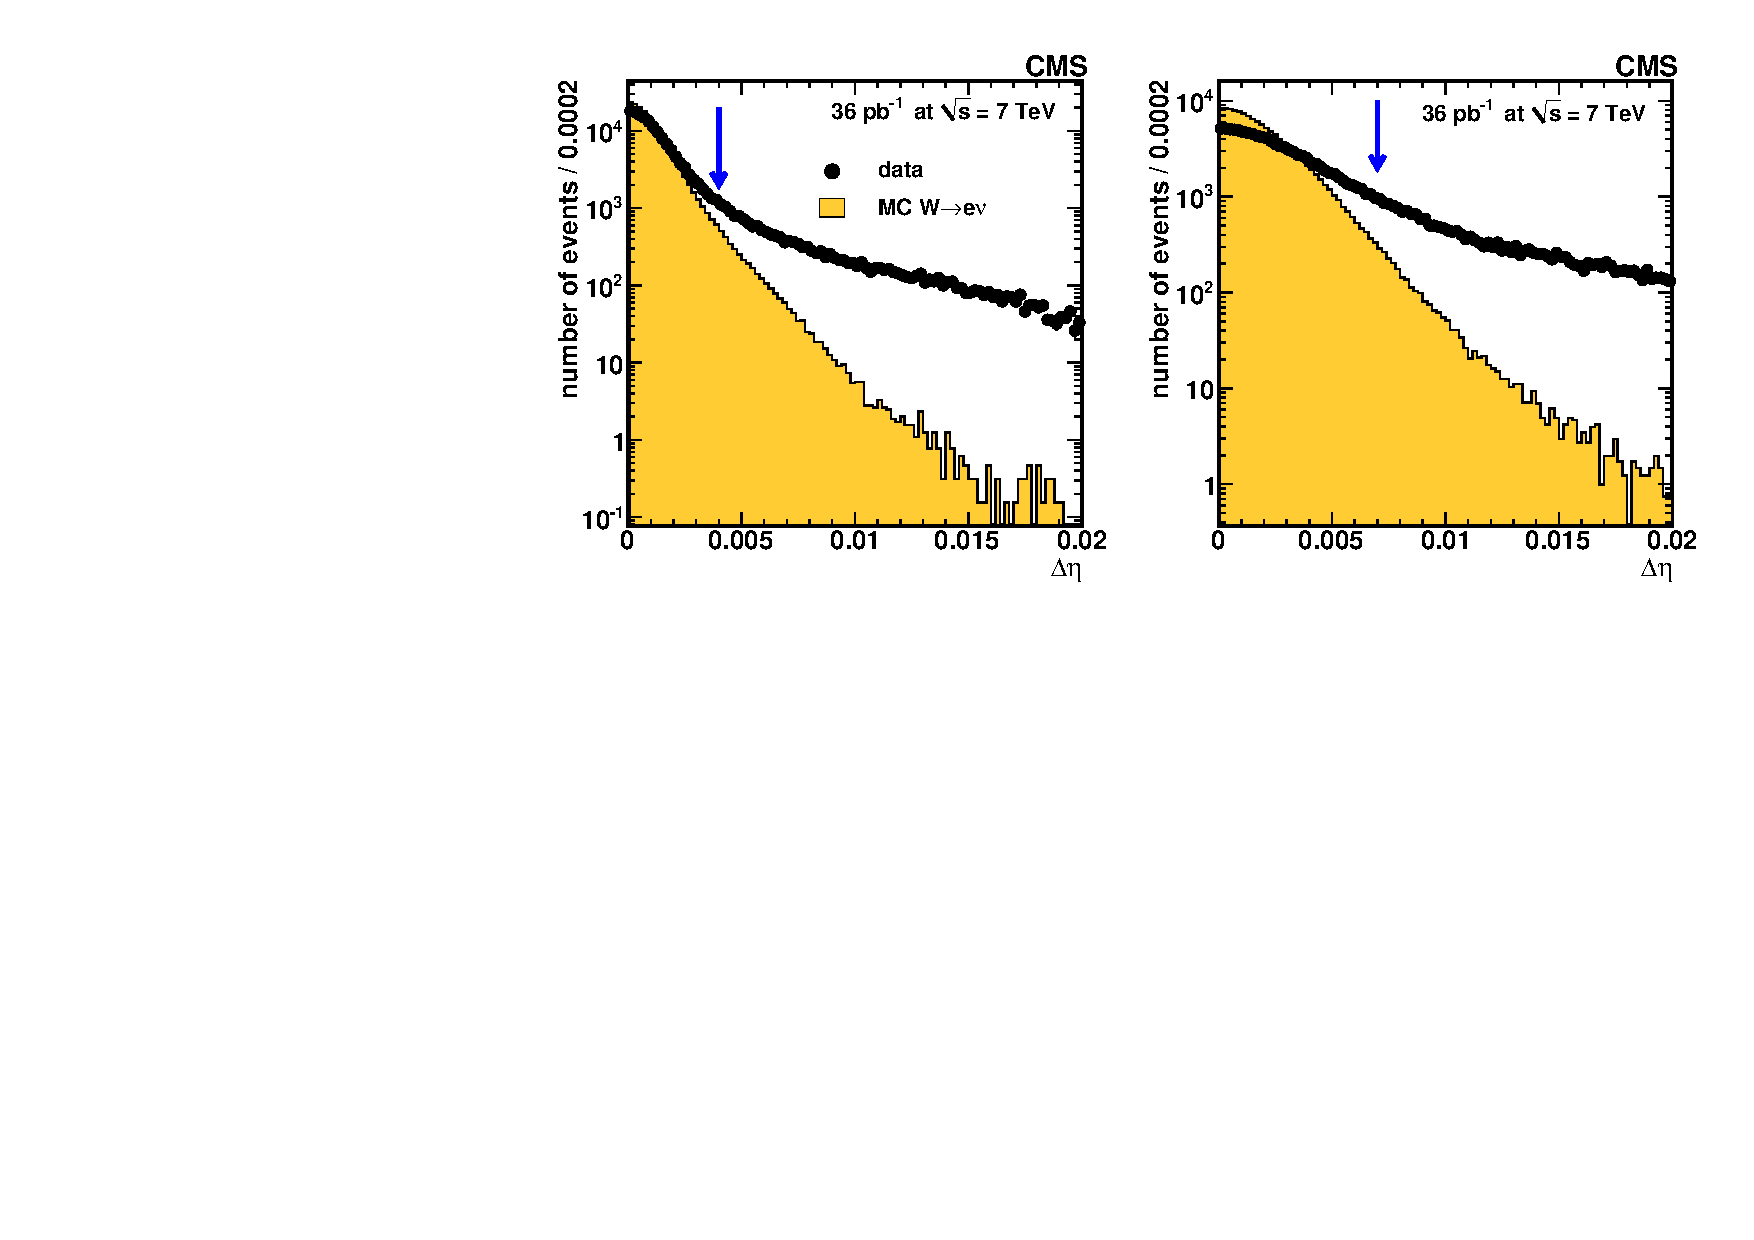
\includegraphics[width=0.68\textwidth]{figs/deta.pdf}
   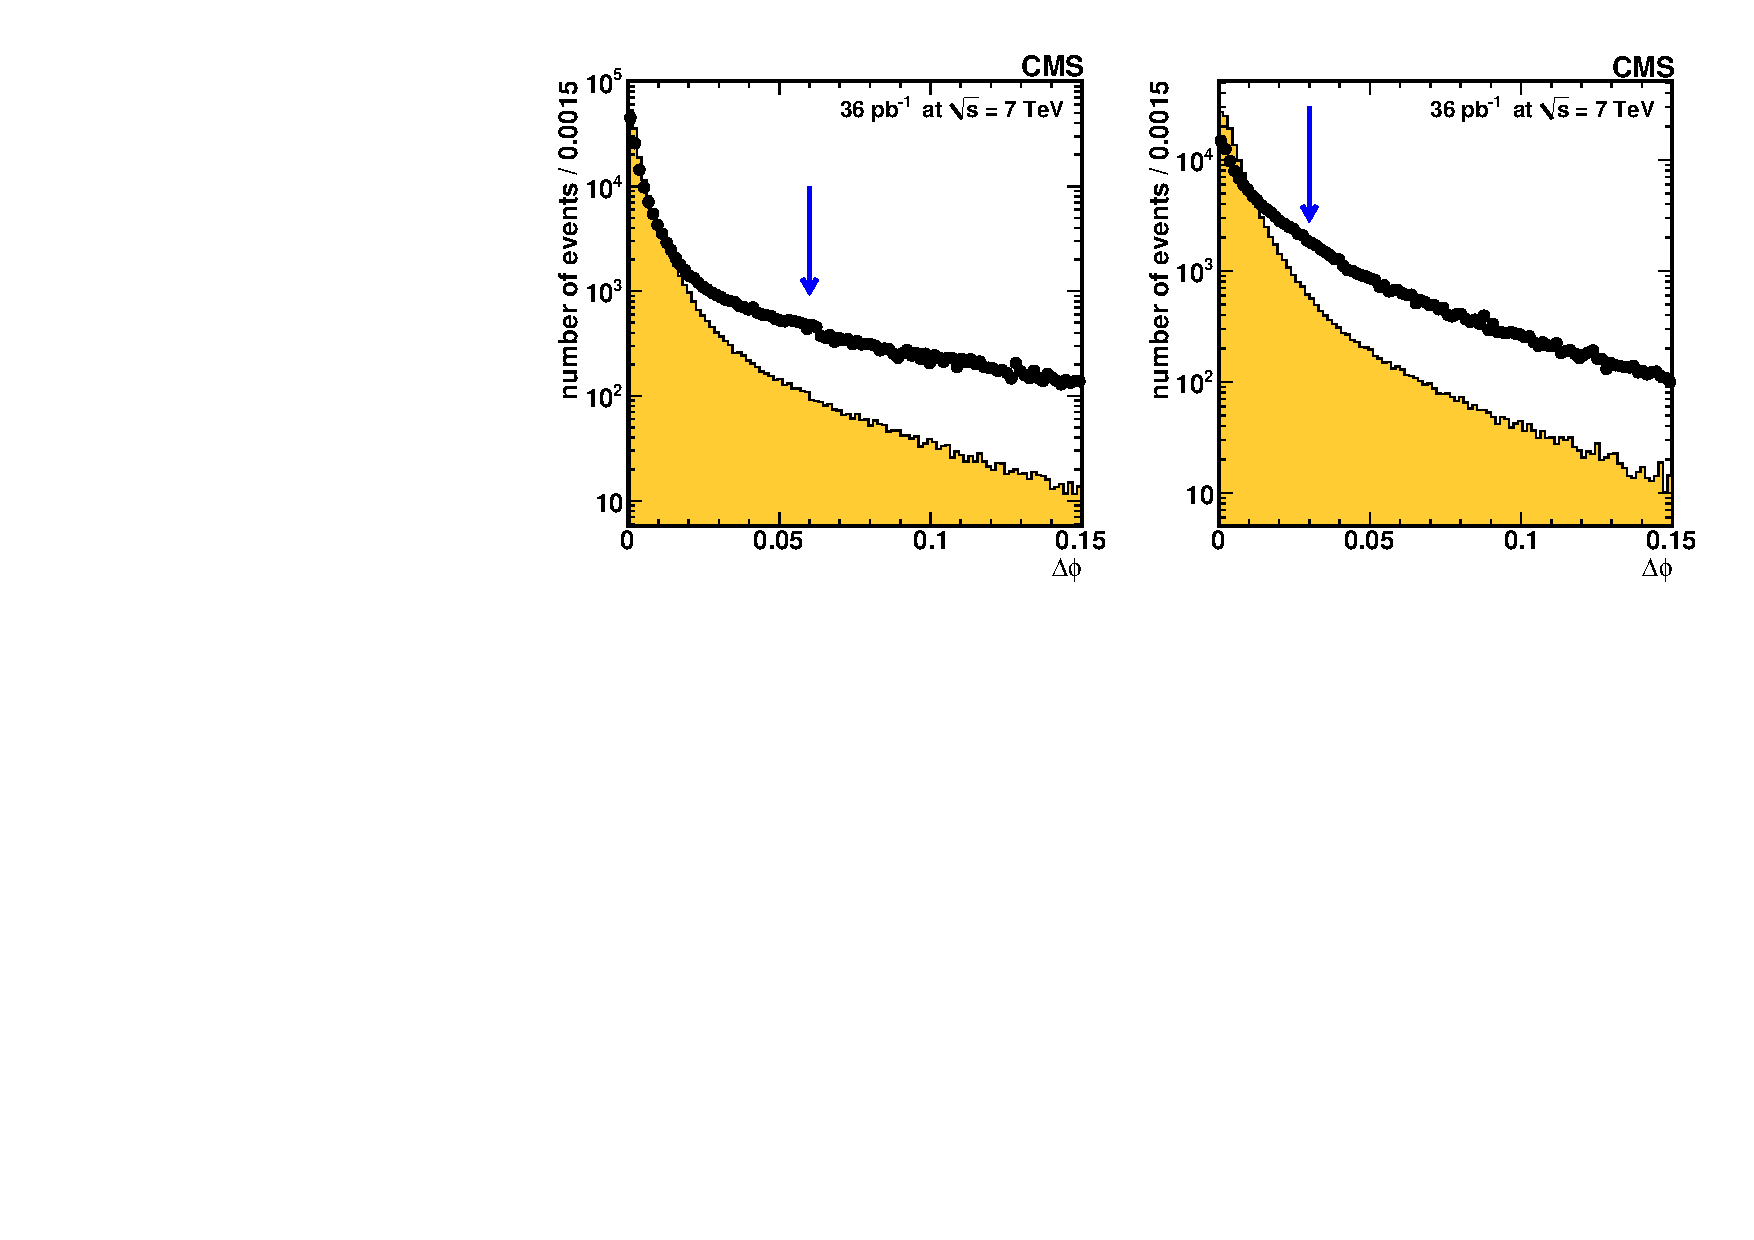
\includegraphics[width=0.68\textwidth]{figs/dphi.pdf}
   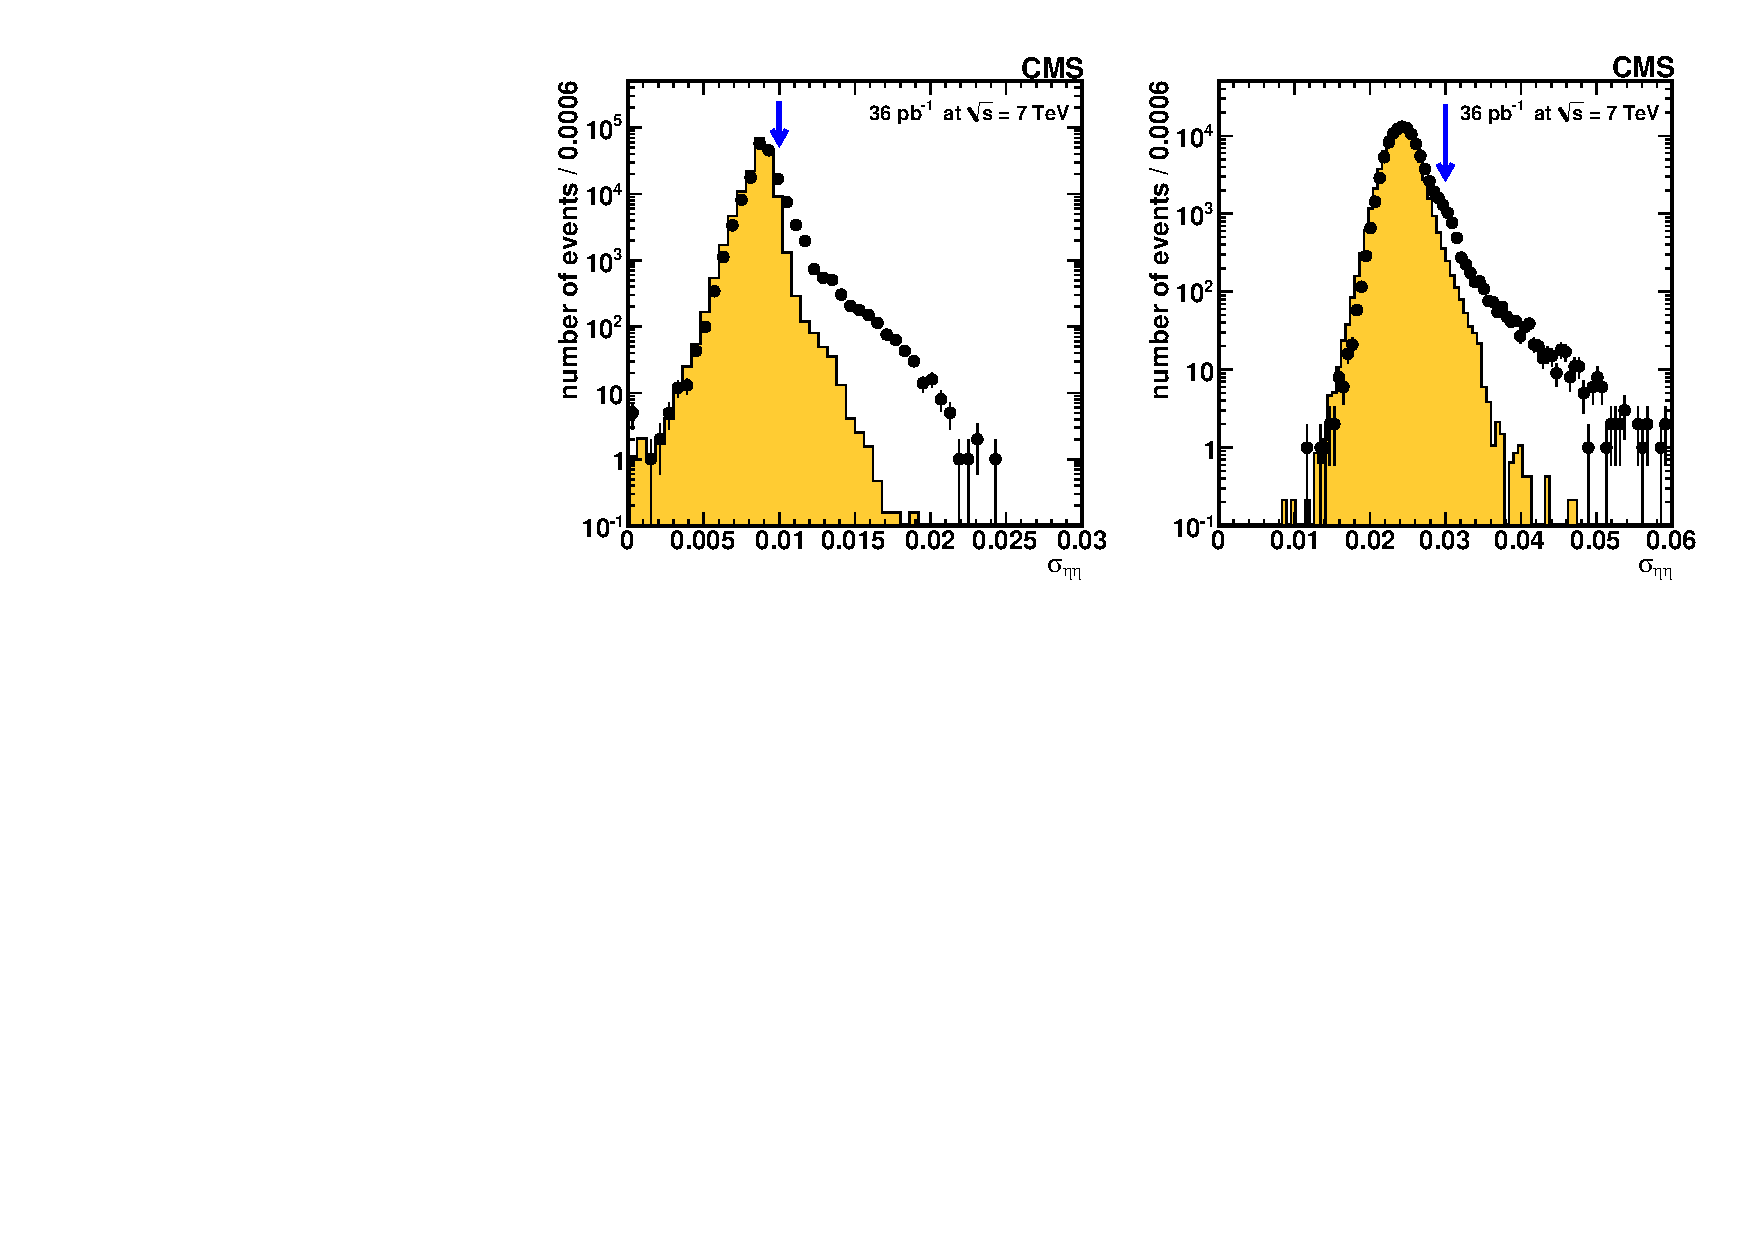
\includegraphics[width=0.68\textwidth]{figs/sihih.pdf}
   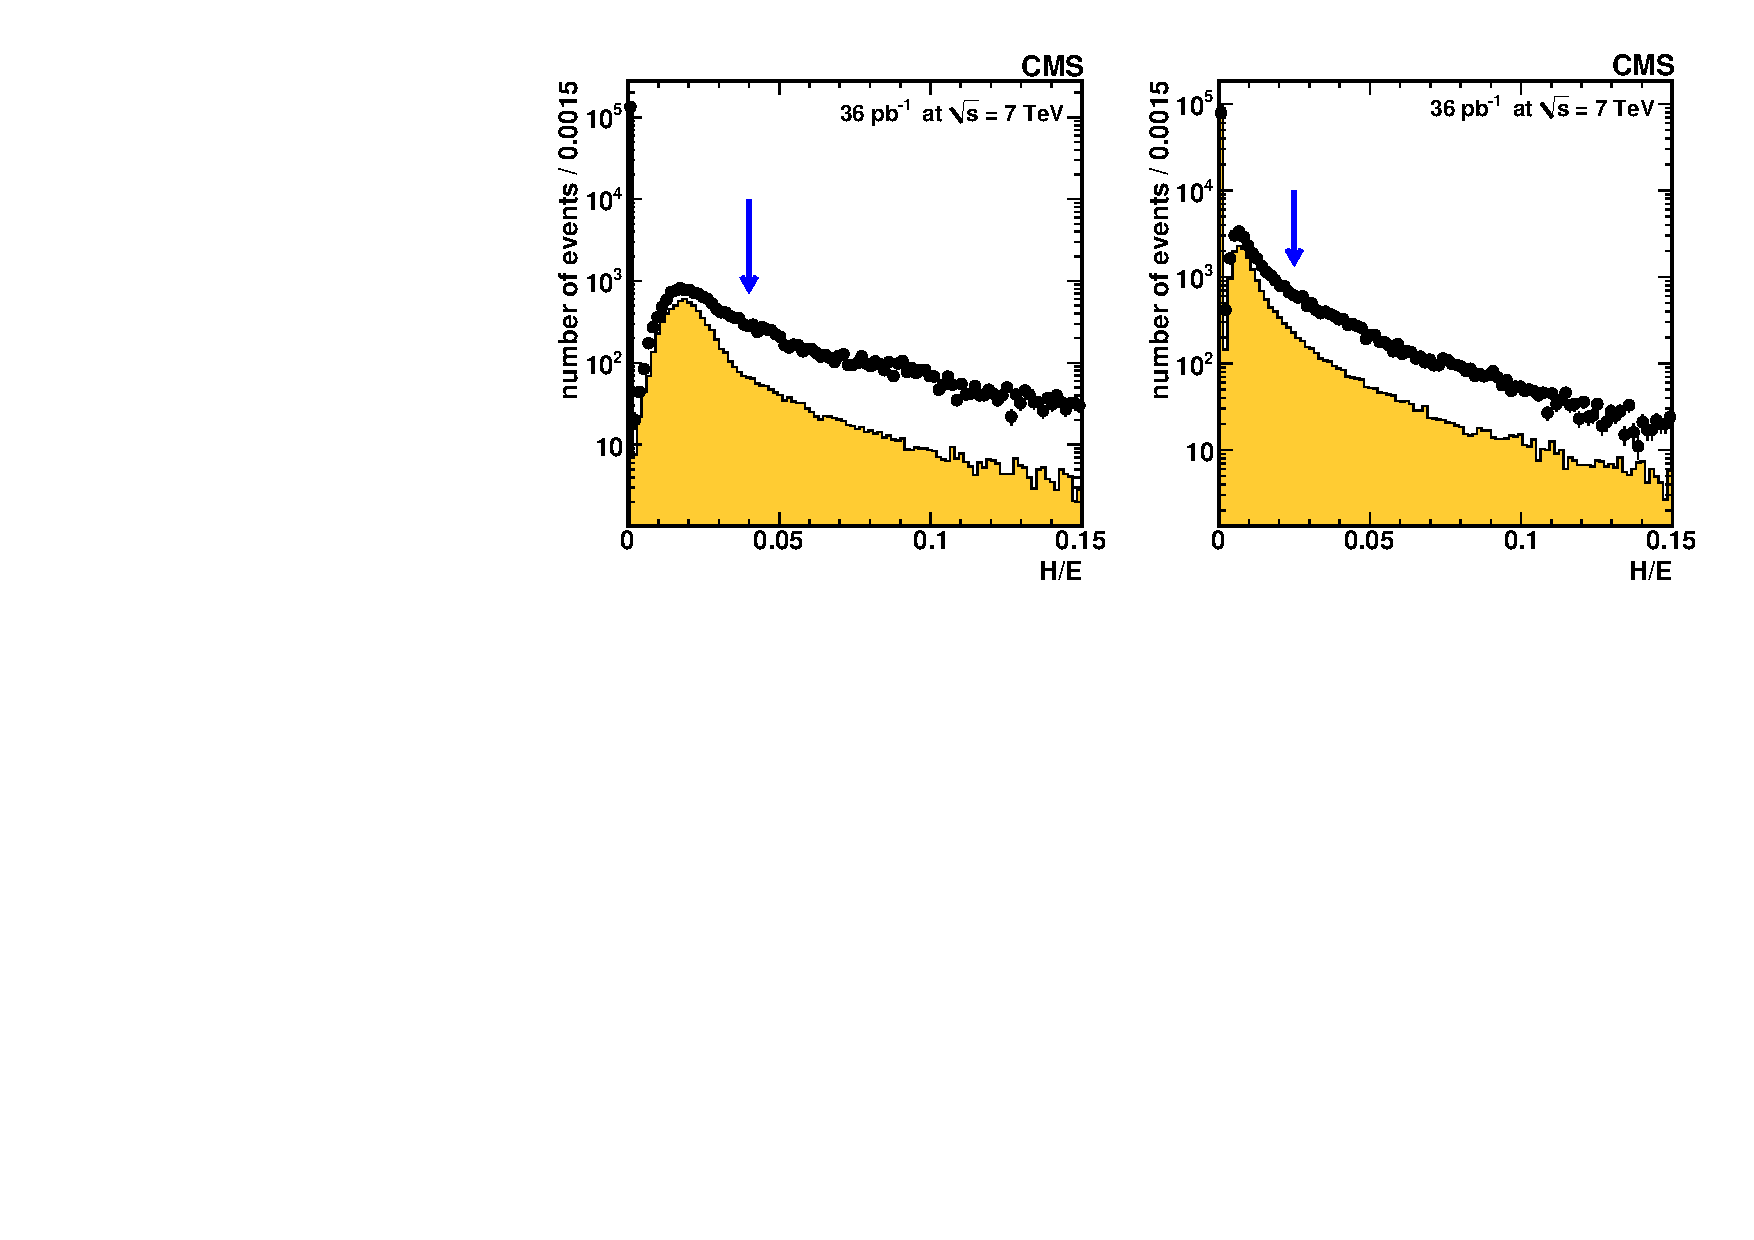
\includegraphics[width=0.68\textwidth]{figs/hoe.pdf}
   \caption{ \label{fig:WenuSelection1}
Distributions of the electron identification variables $\Delta\eta$, $\Delta\phi$, $\sigma_{\eta\eta}$, 
and $H/E$ for data (points with the error bars), for EB (left) and EE (right).
For illustration the simulated $\Wen$ signal (histograms), normalized to the number of events
observed in data, is superimposed.
These distributions are obtained after applying all 
the tight requirements on the selection variables, except that on the presented
variable. The tight requirement on that variable is indicated with an arrow. }
  \end{center}
\end{figure}
%%%%%

%%%%%
\begin{figure}[htbp]
  \begin{center}
   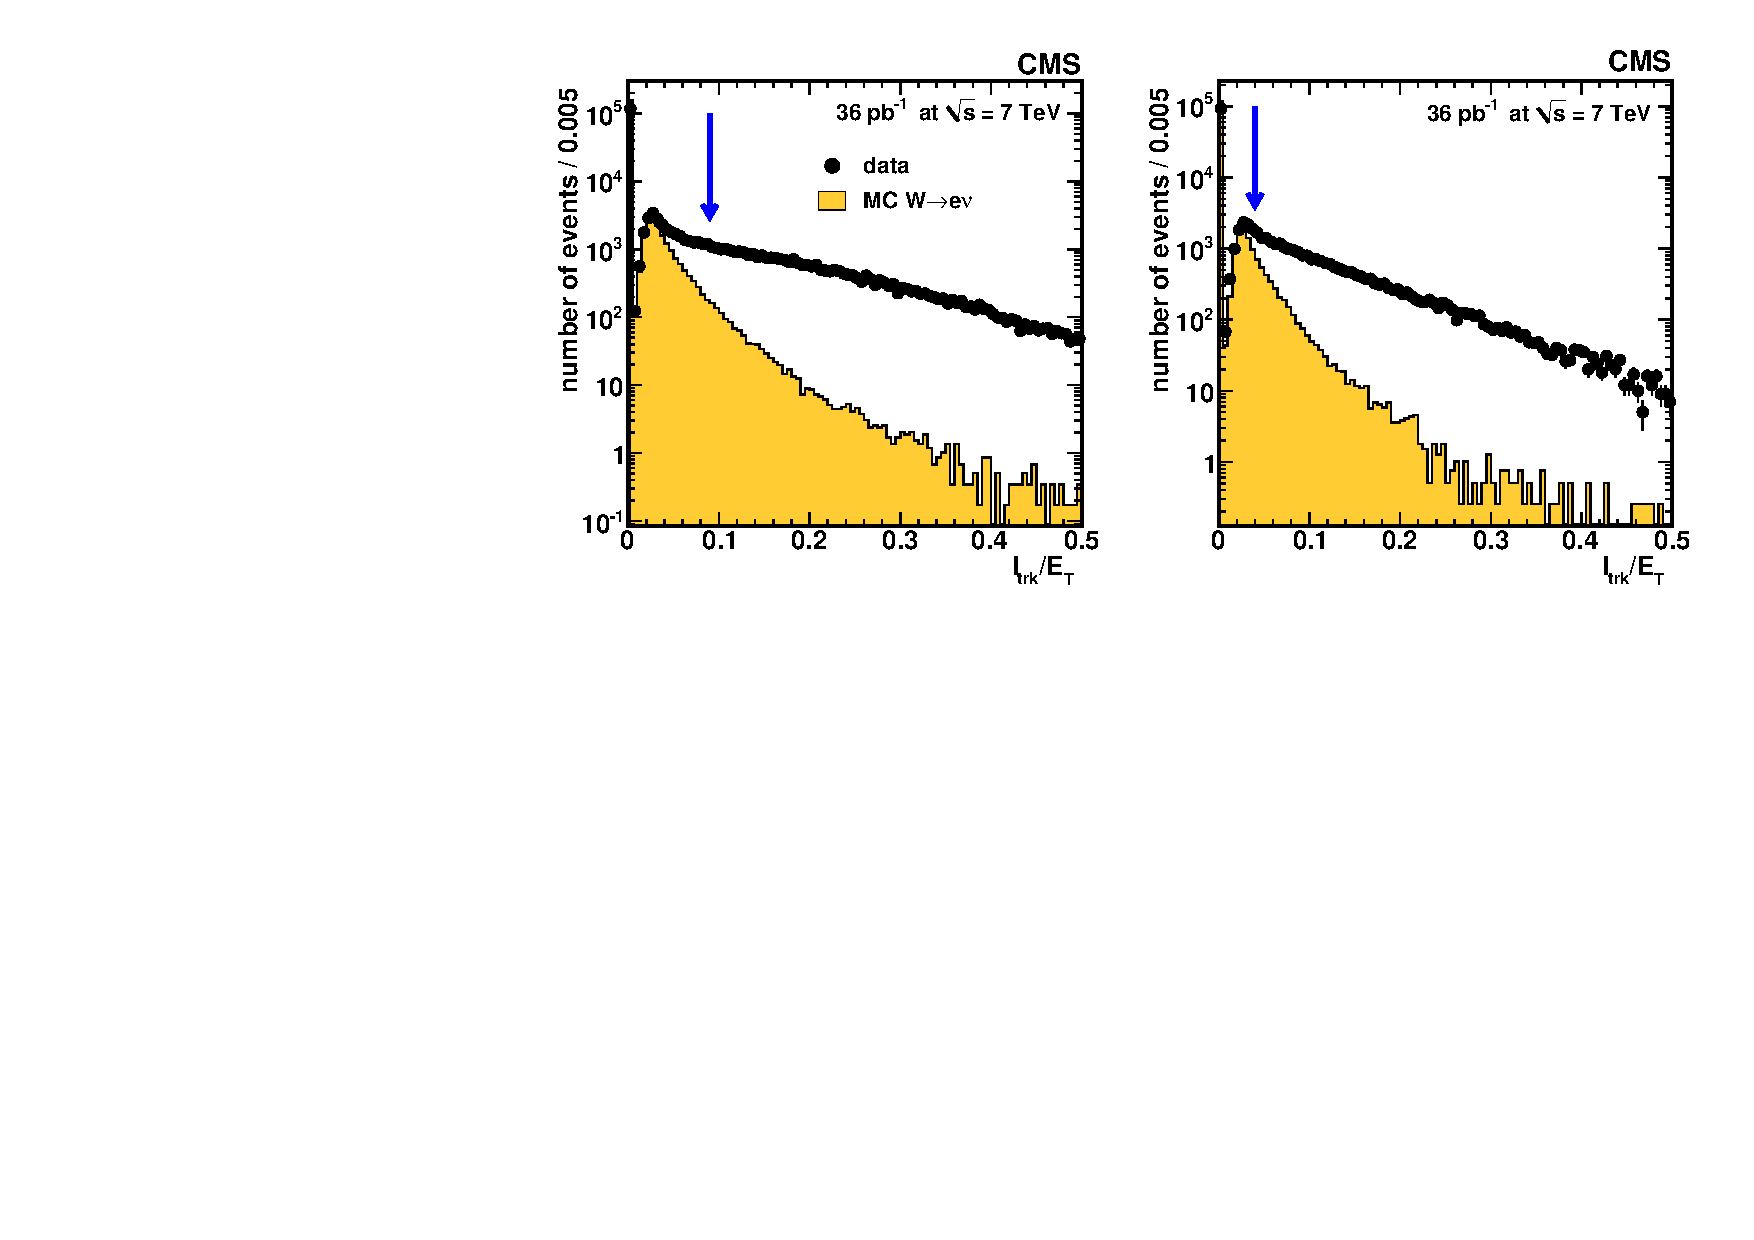
\includegraphics[width=0.68\textwidth]{figs/tkiso.pdf}
   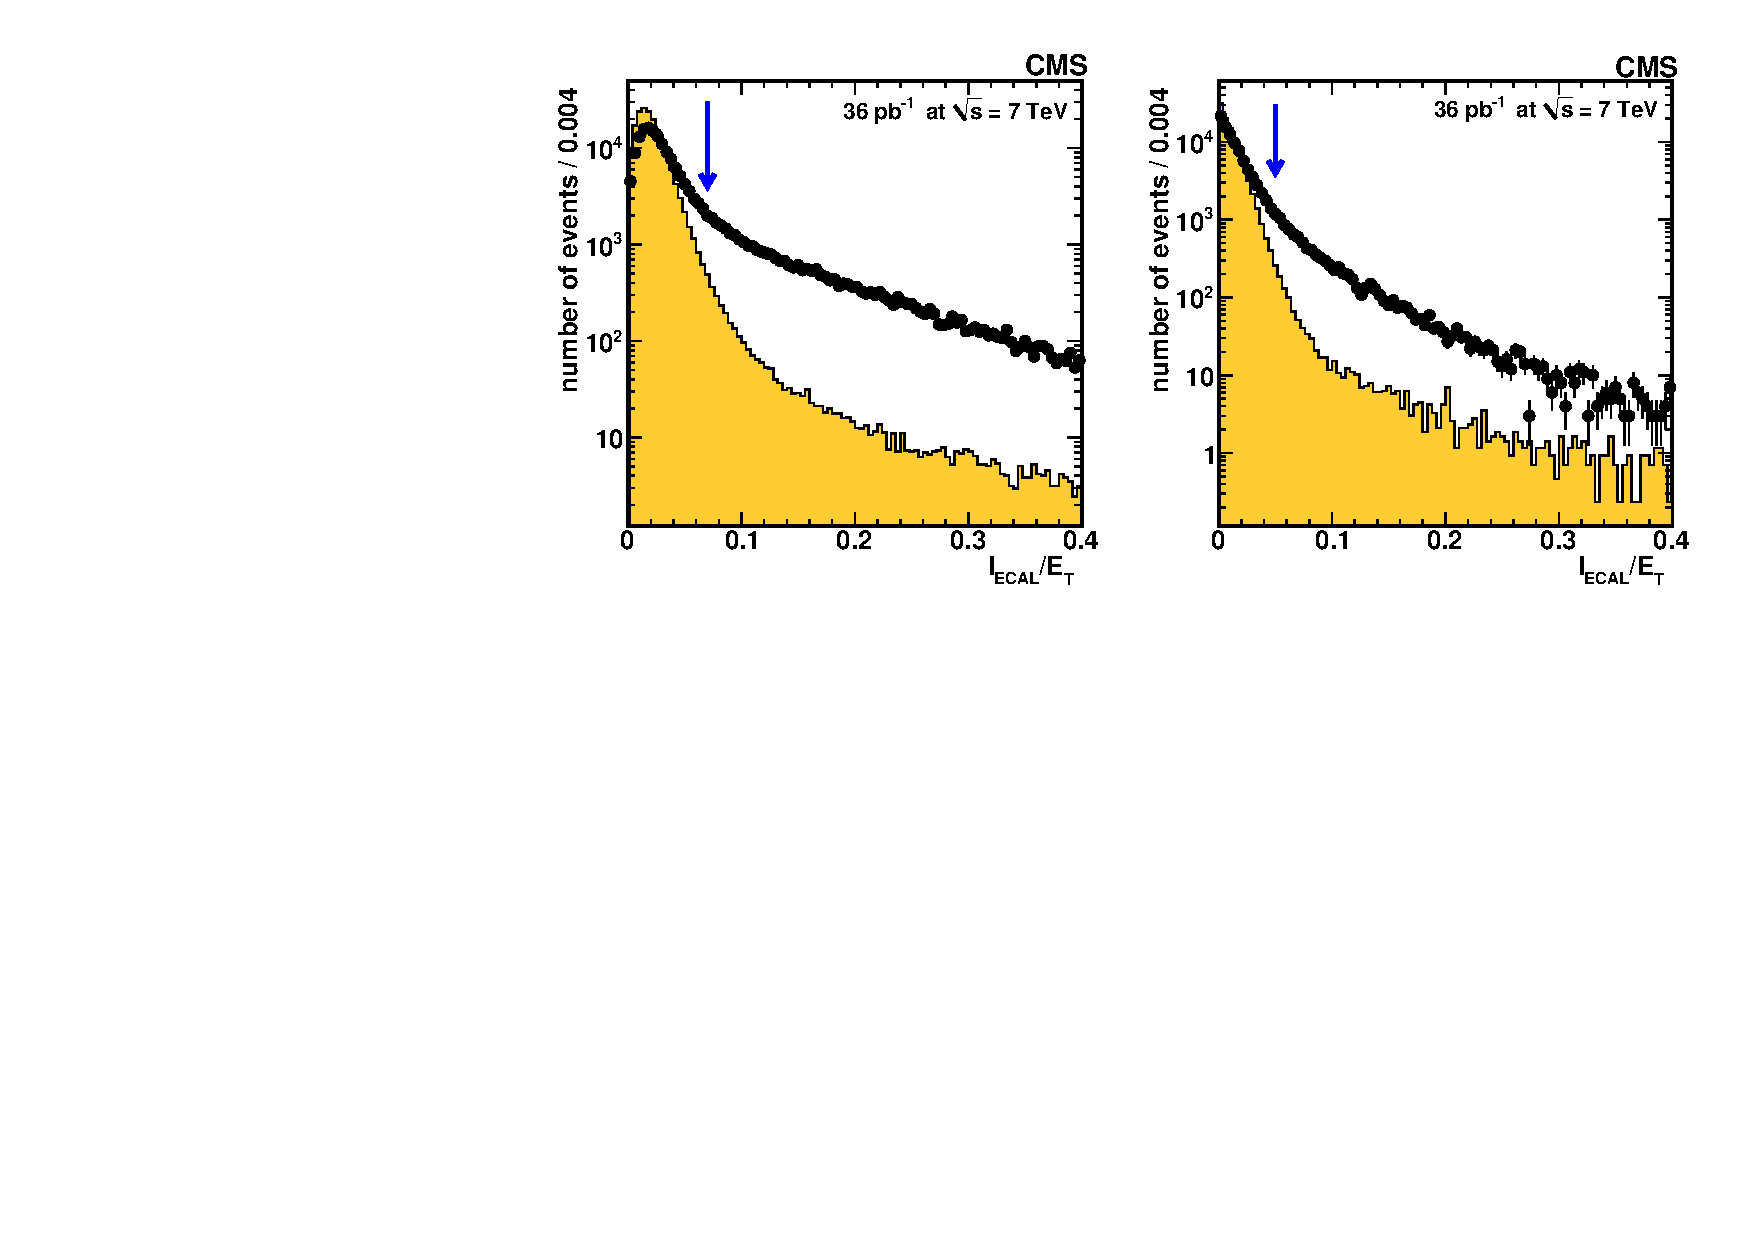
\includegraphics[width=0.68\textwidth]{figs/ecaliso.pdf}
   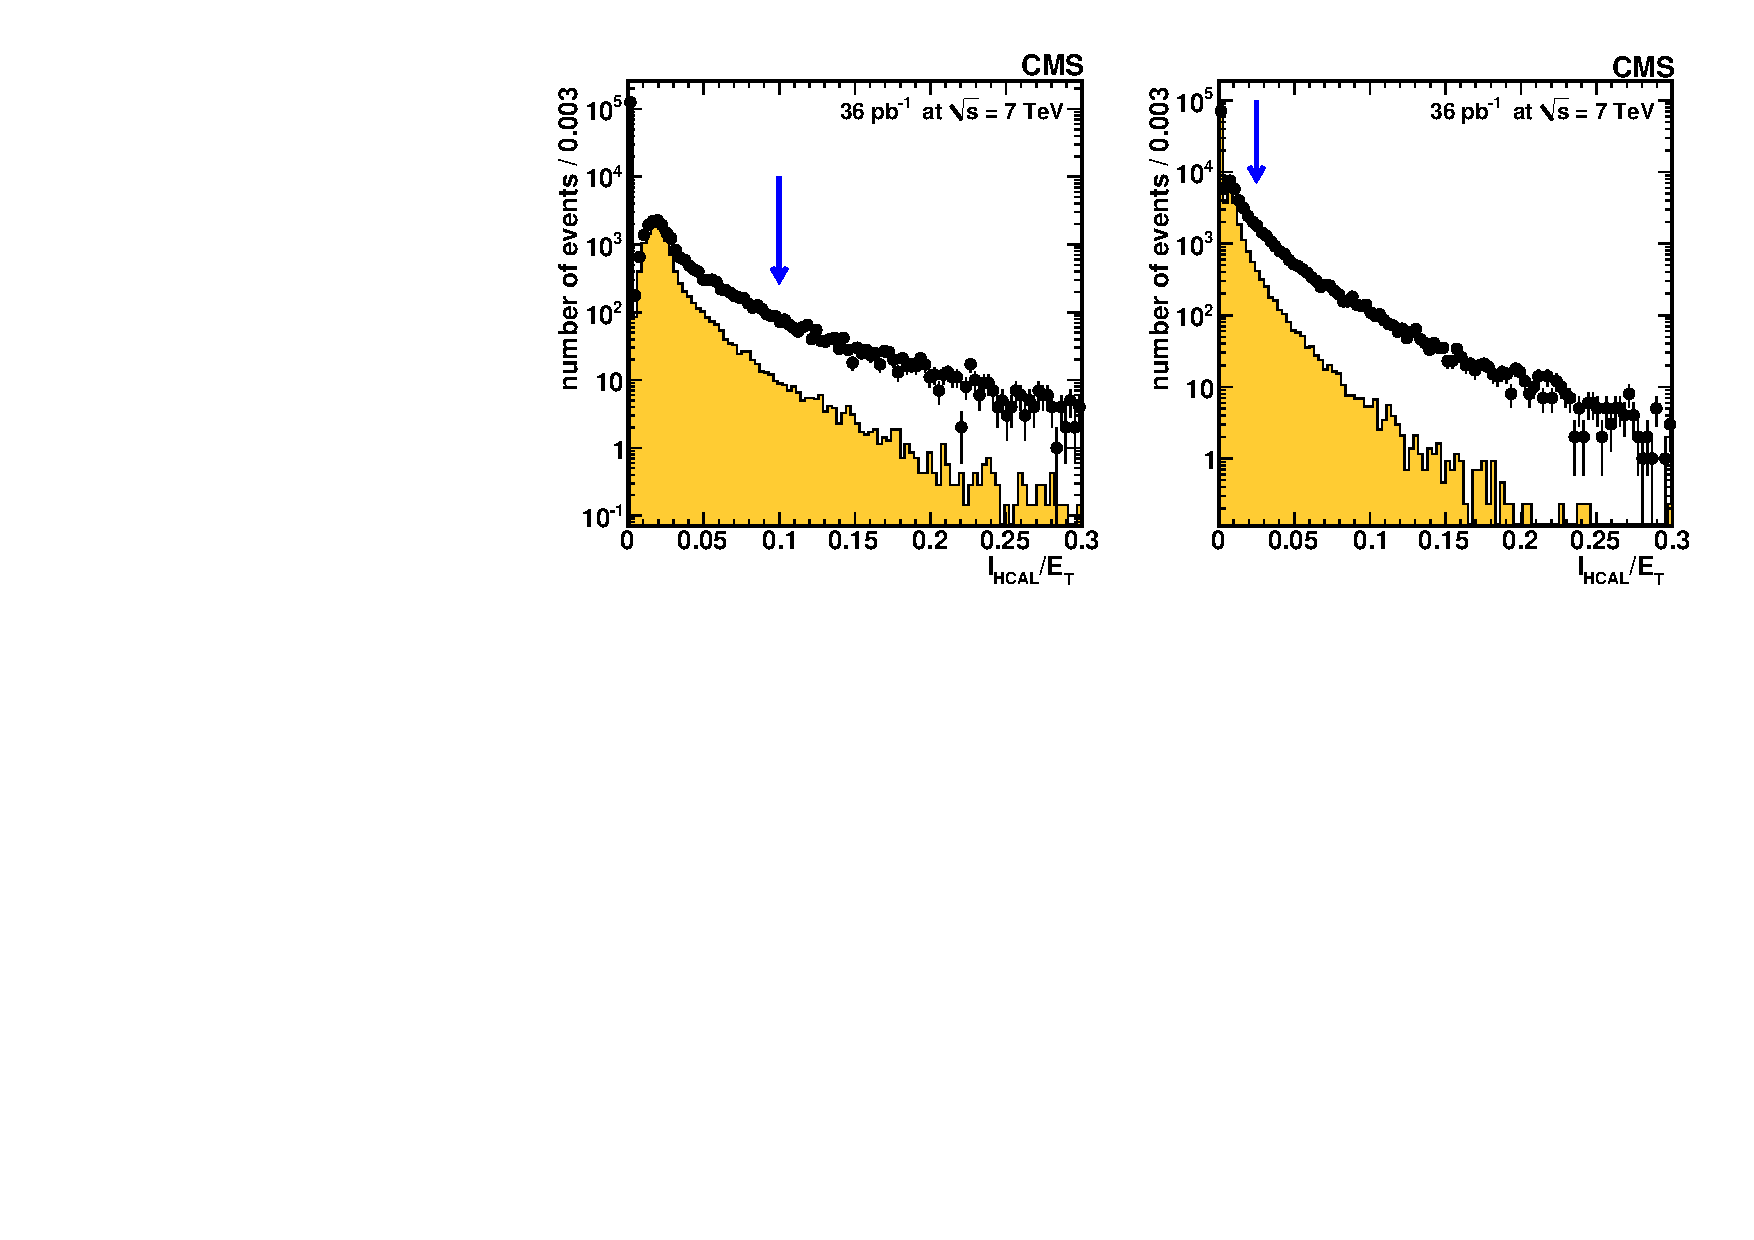
\includegraphics[width=0.68\textwidth]{figs/hcaliso.pdf}
   \caption{ \label{fig:WenuSelection2}
Distributions of the electron isolation variables $\ITRK/\Et$, $\IECAL/\Et$, and $\IHCAL/\Et$
for data (points with the error bars), for EB (left) and EE (right).
For illustration the simulated $\Wen$ signal (histograms), normalized to the number of events
observed in data, is superimposed.
These distributions are obtained after applying all
the tight requirements on the selection variables, except that on the presented
variable. The tight requirement on that variable is indicated with an arrow. }
  \end{center}
\end{figure}
%%%%%

The radiated photons may convert close to the
original electron trajectory, leading to charge misidentification.
Three different methods are used to determine the electron charge. First, the electron 
charge is determined by the signed curvature of the associated GSF track. Second, the charge 
is determined from the associated trajectory reconstructed in the silicon tracker using a 
Kalman Filter algorithm~\cite{KF}. Third, the electron charge is determined based on the azimuthal 
angle between the vector joining the nominal interaction point and the ECAL cluster 
position and the vector joining the nominal interaction point and innermost hit of the GSF track. 
The electron charge is determined from the two out of three charge estimates that are in agreement.
The electron charge misidentification rate is measured in data using the $\Zee$ data
sample to be within 0.1$\%$--1.3$\%$ in EB and 1.4$\%$--2.1$\%$ in EE, increasing with
electron pseudorapidity.


Events are selected if they contain one or two electrons having $\Et>25~\gev$ 
for the $\Wen$ or the $\Zee$ analysis, respectively. 
For the  $\Zee$ selection there is no requirement on the charges of the electrons.
The energy of an electron candidate with $\Et>25~\gev$ is 
determined by the ECAL cluster energy, while its momentum direction is determined by 
that of the associated track. 

Particles misidentified as electrons are suppressed by requiring that the $\eta$ and $\phi$ coordinates
of the track trajectory extrapolated to the ECAL match those
of the ECAL cluster permitting only small differences ($\Delta\eta$, $\Delta\phi$) 
between the coordinates, by requiring a narrow ECAL cluster width in $\eta$ ($\sigma_{\eta\eta}$), 
and by limiting the ratio of the hadronic energy $H$ to the electromagnetic 
energy $E$ measured in a cone of $\Delta R = 0.15$ around the ECAL cluster direction.
More details on the electron identification variables can be found in Refs.~\cite{EGMid,PhotonQCD}. 
Electron isolation is based on requirements on the three isolation 
variables $\IHCAL/\Et$, $\IECAL/\Et$, and $\ITRK/\Et$.

\par
Electrons from photon conversions are suppressed by requiring the 
reconstructed electron track to have at least one hit in the innermost pixel layer.
Furthermore, electrons are
rejected when a partner track is found that is consistent with a
photon conversion, based on the opening angle and the separation in
the transverse plane at the point where the electron and partner
tracks are parallel.

The electron selection criteria were obtained
by optimizing signal and background levels according to
simulation-based studies. The optimization was done for EB
and EE separately.  

Two sets of electron selection criteria are considered: 
a tight one and a loose one.
Their efficiencies, from simulation studies based on $\Wen$ events, are
approximately 80$\%$ and 95$\%$, respectively. These efficiencies correspond 
to reconstructed electrons within the geometrical and kinematic 
acceptance, which is defined in Section~\ref{sec:acceptance}.  
The tight selection criteria give a purer sample of prompt 
electrons and are used for both the $\Wen$ and $\Zee$ analyses.
The virtue of this choice is to have consistent electron definitions 
for both analyses, simplifying the treatment of systematic 
uncertainties in the $\mathrm{W}/\mathrm{Z}$ ratio measurement. 
In addition, the tight working point, applied to both electrons
in the $\Zee$ analysis, reduces the QCD backgrounds to a negligible level.
%%The values of the cuts for the tight and "loose" selection sets are 
%%listed in Table~\ref{tab:electron_cuts}.
%%%%% GD
Distributions of the selection variables are shown in Figs.~\ref{fig:WenuSelection1}
and~\ref{fig:WenuSelection2}.
The plots show the distribution of data together with the simulated signal 
normalized to the same number of events as the data, after applying all 
the tight requirements on the selection variables except the requirement on the displayed
variable. 
%The tight cut on that variable is shown with a vertical line.



For the W analysis, an event is also rejected if there is a second electron 
that passes the loose selection with $\Et > 20~\gev$. This requirement reduces
the contamination from DY events.  
The number of $\Wen$ candidate events selected in the data sample is 
$\WEISAMPLE$, with $\WEPSAMPLE$ positrons and $\WEMSAMPLE$ electrons.

For the Z analysis, two electrons are required within the ECAL acceptance, 
both with $\Et > 25~\gev$ and both satisfying the tight electron selection. 
Events in the dielectron mass region of $60 < m_{\mathrm{ee}} < 120$~GeV are counted.
These requirements select $\ZEESAMPLE$ events.



% \begin{table}[htb]
% \caption{Selection cuts for electrons.}
% \label{tab:electron_cuts}
% \begin{center}
% \begin{tabular}{ | l || c | c || c | c |}
% \hline
%           & \multicolumn{2}{| c ||}{"Loose" e} & \multicolumn{2}{| c |}{tight e} \\
% \hline
%                          & Barrel & Endcap & Barrel & Endcap \\
% \hline \hline
%    $\ITRK/\Et$             & 0.15   & 0.08   & 0.09   & 0.04   \\
% \hline
%    $\IECAL/\Et$              & 2.0    & 0.06   & 0.07   & 0.05   \\
% \hline
%    $\IHCAL/\Et$              & 0.12   & 0.05   & 0.10   & 0.025  \\
% \hline
%    Missing hits $\leq$    & 1      & 1      & 0      & 0      \\
% \hline
%    Dcot                  & $-$    & $-$    & 0.02   & 0.02   \\
% \hline
%    Dist                  & $-$    & $-$    & 0.02   & 0.02   \\
% \hline
%    $\sigma_{\eta\eta}$   & 0.01   & 0.03   & 0.01   & 0.03   \\
% \hline
%    \DP                    & $-$    & $-$    & 0.06   & 0.03   \\
% \hline
%    \DE                    & 0.007  & 0.01   & 0.004  & 0.007  \\
% \hline
%    $H/E$                  & 0.15   & 0.07   & 0.04   & 0.025  \\
% \hline
% \end{tabular}
% \end{center}
% \end{table}







%\subsection{Muons \label{sec:muonId}}

%Muon used in this analysis are selected according to the
%quality criteria studies in
%Events with high-$\Pt$ muons are recorded online using the Level-1 muon
%trigger and the High-Level Trigger (HLT), which requires muons within $|\eta| < 2.1$ and
%with a thresholds of $\Pt>9 \GeVc$ or $\Pt>15 \GeVc$, according to the running periods. 
Muons must be identified by two different algorithms~\cite{MUONPAS}: one proceeds from 
the inner tracker outwards (``tracker muons''), the other one starts from 
segments in the muon chambers and proceeds inwards (``global muons''). 
Decays in flight of hadrons and punch-through are reducing a cut of $\chi^2/ndof < 10$ 
on a global fit containing tracker and muon detector hits. 
In order to ensure a precise estimate of momentum and impact parameter 
%(the muon momentum resolution is dominated by the inner tracker detector
%for the tranverse momentum range interesting for this measurement)
only tracks with more than 10 hits and at least one hit in the pixel detector are used. 
We require at least two levels of muon stations in the measurement, 
to ensures a good quality momentum estimate at trigger level, and
to further suppresses remaining fake muon candidates.
%For the $\Zmm$ analysis we minimize the cross-corrlation between tracker and muon 
%detectors by drop the $\chi^2/{\mathrm{ndof}}$ and 
%the request that the muon is found by the tracker algorithm.
Cosmics are rejected by requiring a transverse impact parameter distance to the beam spot
position of less than 2 mm.



%\subsubsection{$\Wen$}

The event selection requirements for $\Wen$ are then as follows:
\begin{enumerate}
\item
one identified electron within acceptance, satisfying the WP80 set
of identification and isolation criteria,
\item
if a second electron candidate with $\Et > 20~\gev$, within ECAL fiducial 
and satisfying looser identification and isolation criteria (WP95) is present
in the event, the event is rejected.
\end{enumerate}

The number of $\Wen$ candidate events selected
in the data sample is
$\WEISAMPLE$, with
$\WEPSAMPLE$ positrons and
$\WEMSAMPLE$ electrons.


%\subsubsection{$\Wmn$ Event Selection}
\label{sec:WmnSel}

% $\Wmn$ events are characterized by a high-$\Pt$, isolated muon,
% together with a significant amount of missing $\Et$, due to the
% presence of a neutrino in the final-state, that escapes undetected.

The first step in the $\Wmn$ candidate selection is to
reject those events having two global muons satisfying: $\Pt(\mu_1) >
20~\GeV$ and $\Pt(\mu_2) > 10~\GeV$, where $\Pt(\mu_1)$ is the
highest muon $\Pt$ and $ \Pt(\mu_2)$ is the second highest muon $\Pt$
in the event, in order to minimize the contamination from DY
events.

Events with a good quality muon, as described in Section~\ref{sec:muonid},
in the fiducial volume $|\eta|<2.1$, and with a transverse momentum
higher than $25~\GeV$ are kept.
Relative combined isolation variable (see Section~\ref{sec:isolation}) is used to evaluate the level of activity around the
muon. Isolation distribution of the experimental data, together with the simulation expectations, is shown in
Fig.~\ref{figure:Wmunu_iso}. The muon is considered to be isolated if $\IRelComb < 0.1$.
Events with $\IRelComb > 0.2$ are mainly coming from QCD background, and are be used as 
control sample (see Section~\ref{sec:WQCDbkg}).

\begin{figure}[htb] {\centering
    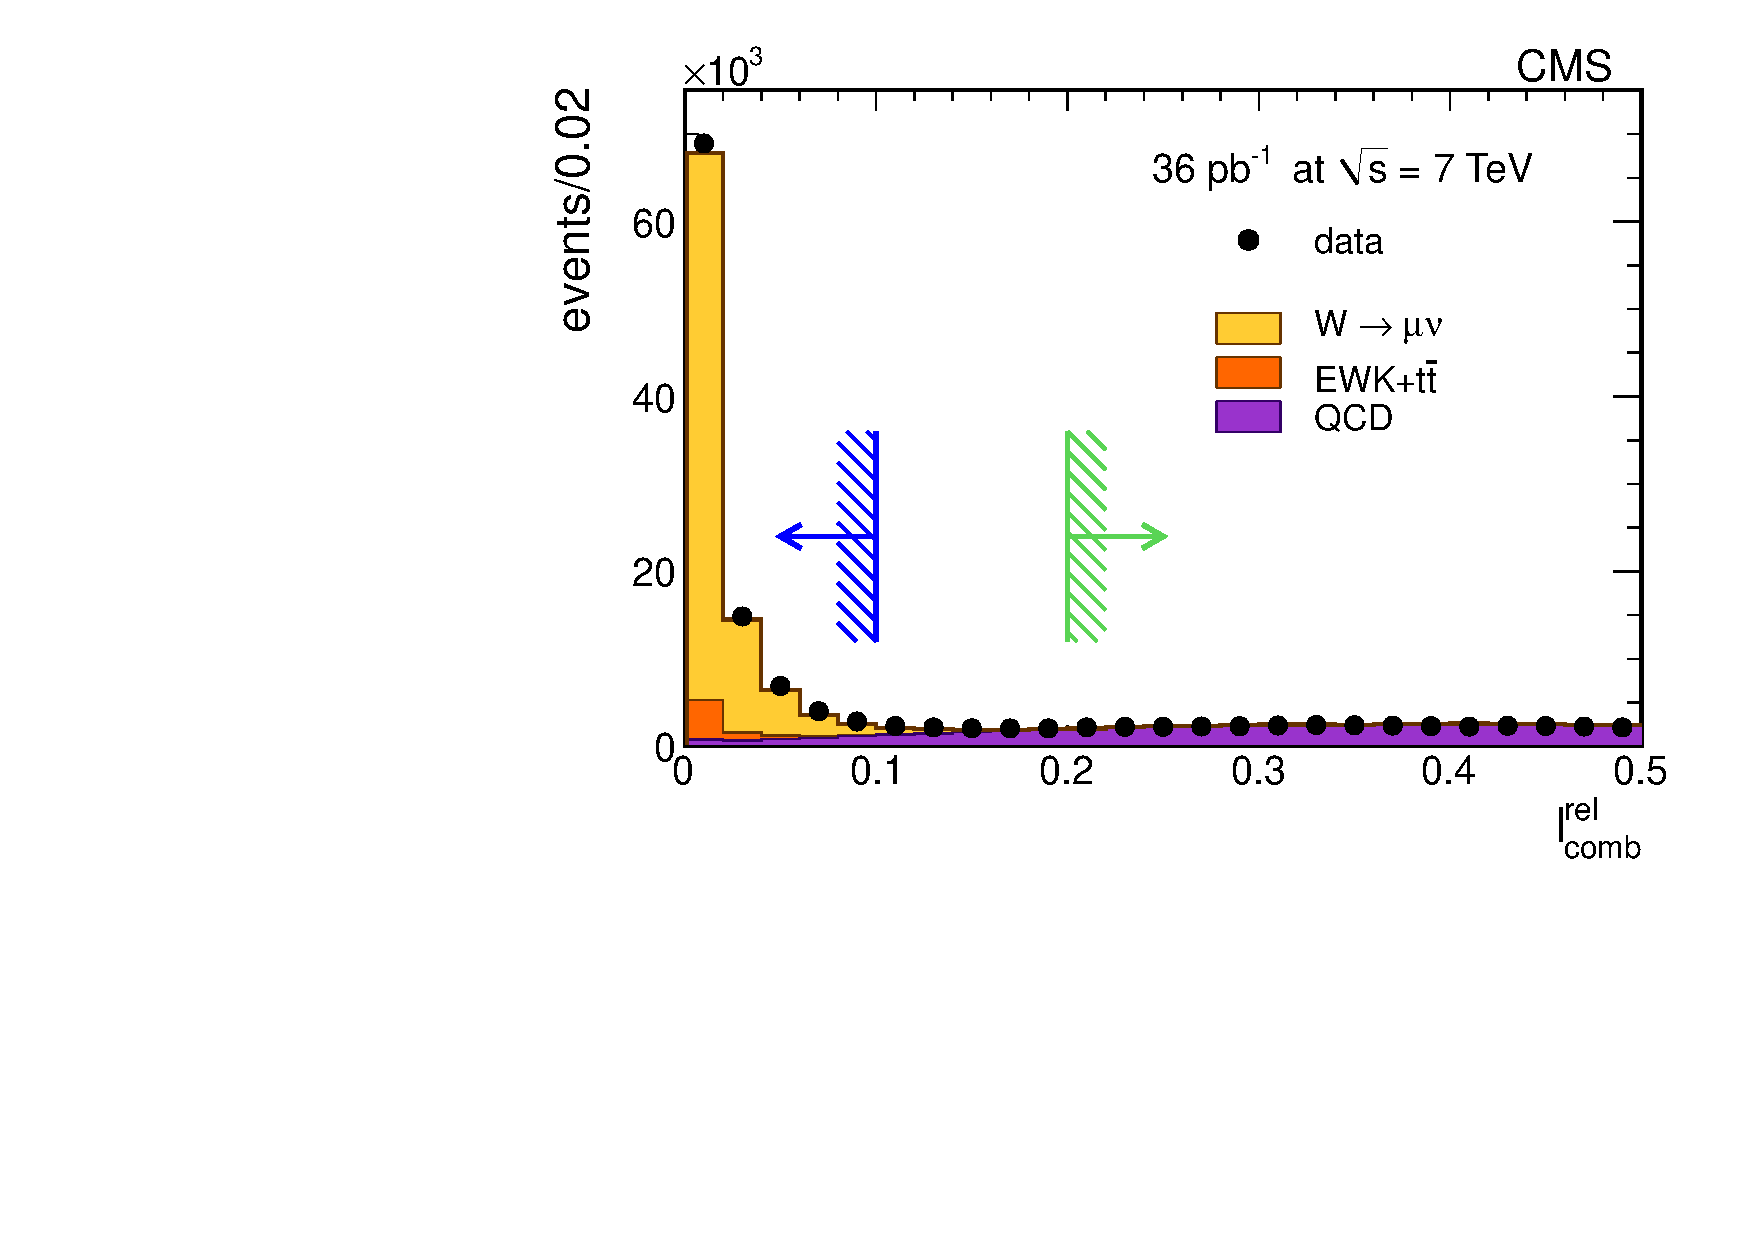
\includegraphics[width=8cm]{figs/Wmunu_isolation.pdf}
    \caption{Isolation distribution of $\Wmn$ candidates with a good quality muon of $\Pt>25~\GeV$ in the fiducial region $|\eta|<2.1$.
Dots represent the data and the solid histograms the contribution from the different SM processes.
The superimposed arrows represent the signal selection requirement (red
arrow, $\IRelComb<0.1$) and selection of the QCD-enriched
control sample (green arrow, $\IRelComb>0.2$).
}
    \label{figure:Wmunu_iso}}
\end{figure}


% The breakdown of the data reduction at the different stages of the
% selection is summarized in Table~\ref{table:Wmunu_selection} both for
% the total sample of muon events, and split by the muon charge.
% %%%%%%%%
% \begin{table}[!ht] 
% \begin{center}
% \begin{tabular}{|c||c|c|c|} \hline
% {Event Sample}                           & Events with $\mu^\pm$ &  Events with $\mu^+$ & Events with $\mu^-$ \\ \hline \hline
% {Candidates}                             &         6395420       &      1812890        &      1677349      \\
% {Triggered}                              &         3174720       &      1644727        &      1529995      \\
% {DY Rejection}                           &         3133420       &       1623994       &      1509425      \\
% {Muon ID}                                &         2618199       &       1346297       &      1271902      \\
% {$|\eta|<2.1$}                           &         2527047       &       1298777       &      1228270      \\
% {$\Pt > 25 \GeV$}                       &          412266       &        222080       &      190186       \\
% $\IRelComb<0.1$                         &          166457       &         97533       &       68924       \\ \hline
% \end{tabular}
% \caption{Data reduction at every step of the selection process.
% Number of events are given for the whole muon data sample, as well as separated by the muon charge.}
% \label{table:Wmunu_selection}
% \end{center}
% \end{table}

After the selection process just described, 166457 events are selected,
97533 of them with a positive charged muon and 68924 with a negative
charged muon.



%\subsection{$\Zll$ Selection}

%
\subsubsection{$\Zee$}


The event selection requirements for $\Zee$ are as follows:
\begin{enumerate}
\item
two electrons within acceptance (as defined above, in Section~\ref{sec:electronId}),
satisfying the WP80 selection,
\item
the dielectron mass must satisfy $60 < m_{\mathrm{ee}} < 120$~GeV.
\end{enumerate}
\par
There is no requirement on the charges of the electrons.
These requirements select \ZEESAMPLE events.



%\input{ZmmSel}
